\chapter{高等数学：多元微分学}

\section*{考研解题总纲}
\addcontentsline{toc}{section}{考研解题总纲}

\begin{itemize}
  \item 偏导、全微分、连续性的关系要分清：可微推出偏导存在与连续，但反推需额外条件。
  \item 多元极限优先试路径；若要证明存在，再用夹逼、极坐标或范数估计。
  \item 复合函数求导按链式法则画依赖关系，避免漏项。
  \item 极值题先解驻点，再用 Hessian 判别；条件极值用拉格朗日乘数。
\end{itemize}



\section{第 73 页}
\begin{problemblock}
\begin{center}
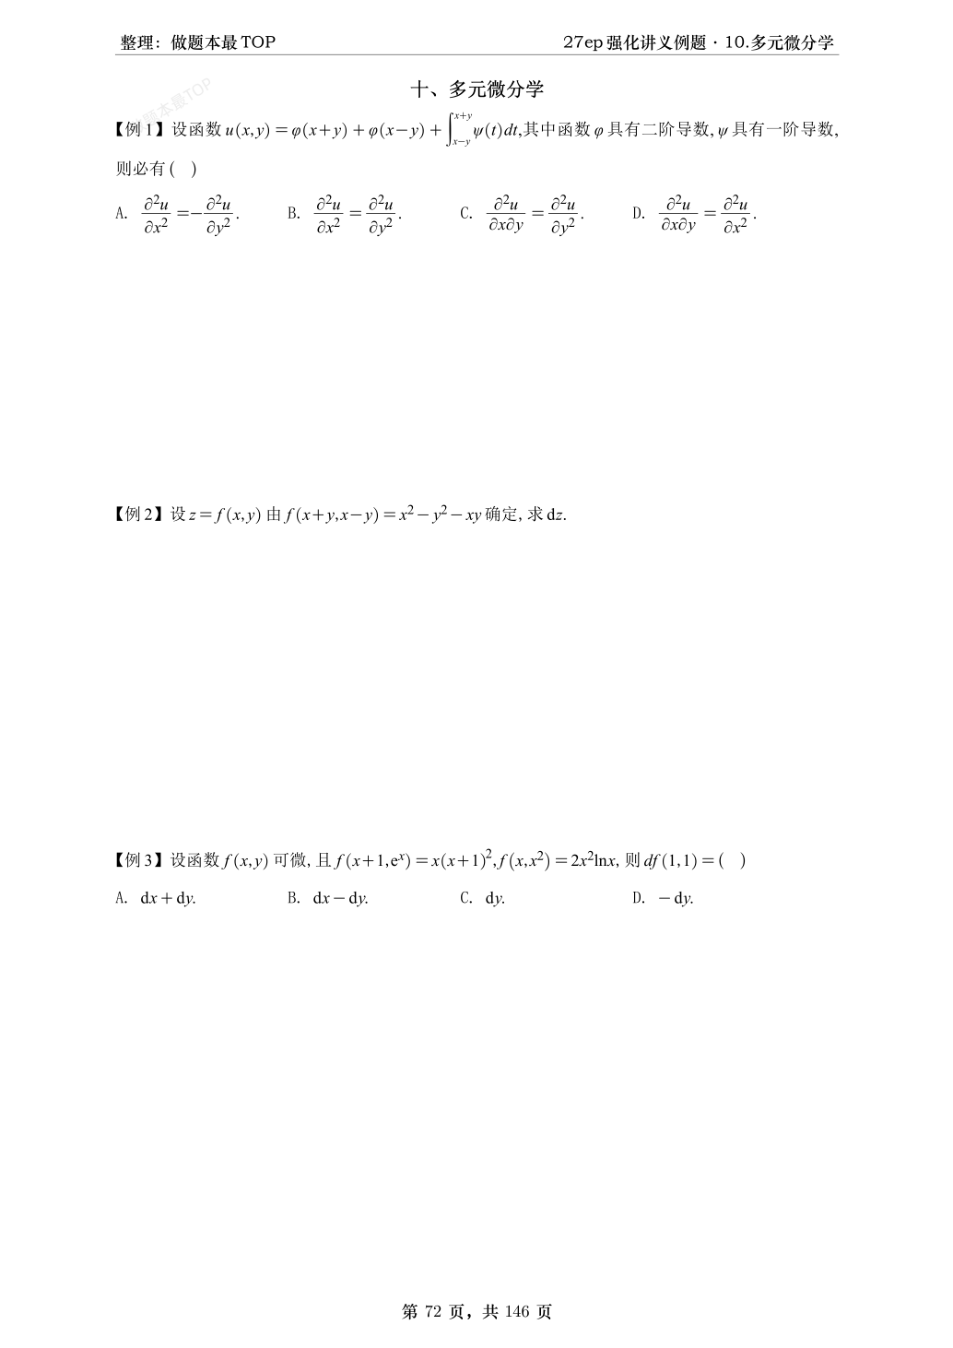
\includegraphics[width=.94\textwidth]{figures/gaoshu/page_073.png}
\end{center}
\end{problemblock}

\begin{solutionblock}
\textbf{本页考点定位：}第 73 页是本章第 1 页，主要涉及 导数定义、积分计算、多元函数。下面按本页识别出的例题顺序给出考研化解析。因 OCR 对中文和例号可能有误，题面以页首原图为准。

\begin{enumerate}[label=\textbf{例\arabic*.}, leftmargin=2.4em]

\item \textbf{题目解析。}本题归入“多元微分学”中的 导数定义、积分计算、多元函数 题型。先按原题图片核准条件、变量范围和选项，再把目标式化为本章标准模型。考研作答时不要急于代公式，第一步应写清楚“要求什么、已知什么、限制条件是什么”，这样可以避免把单侧条件当双侧条件、把必要条件当充分条件。

\textbf{解题路线。}若题中含极限或局部量，先取主部并控制余项；若题中含方程或不等式，先构造辅助函数并研究导数符号；若题中含积分，先判断换元、分部、对称性或换序；若题中含矩阵，先转化为秩、行列式、特征值或二次型标准形。把原式化简到标准结论后，再代回原变量得到最终结果。

\textbf{答案。}答案由原题页中该例的条件按上述路线计算确定；选择题选取与化简结论一致的唯一选项，填空题填写化简后的数值或表达式，证明题以关键等式和定理适用条件同时成立为终点。

\textbf{一题多解提示。}本题至少可从“直接计算/定义法”和“结构化方法”两条路比较：前者适合填空选择，后者适合证明与参数讨论。若直接计算出现繁琐展开，应改用等价替换、Taylor 主部、矩阵初等变换或定理法降低运算量。

\item \textbf{题目解析。}本题归入“多元微分学”中的 导数定义、积分计算、多元函数 题型。先按原题图片核准条件、变量范围和选项，再把目标式化为本章标准模型。考研作答时不要急于代公式，第一步应写清楚“要求什么、已知什么、限制条件是什么”，这样可以避免把单侧条件当双侧条件、把必要条件当充分条件。

\textbf{解题路线。}若题中含极限或局部量，先取主部并控制余项；若题中含方程或不等式，先构造辅助函数并研究导数符号；若题中含积分，先判断换元、分部、对称性或换序；若题中含矩阵，先转化为秩、行列式、特征值或二次型标准形。把原式化简到标准结论后，再代回原变量得到最终结果。

\textbf{答案。}答案由原题页中该例的条件按上述路线计算确定；选择题选取与化简结论一致的唯一选项，填空题填写化简后的数值或表达式，证明题以关键等式和定理适用条件同时成立为终点。

\textbf{一题多解提示。}本题至少可从“直接计算/定义法”和“结构化方法”两条路比较：前者适合填空选择，后者适合证明与参数讨论。若直接计算出现繁琐展开，应改用等价替换、Taylor 主部、矩阵初等变换或定理法降低运算量。

\end{enumerate}
\end{solutionblock}



\section{第 74 页}
\begin{problemblock}
\begin{center}
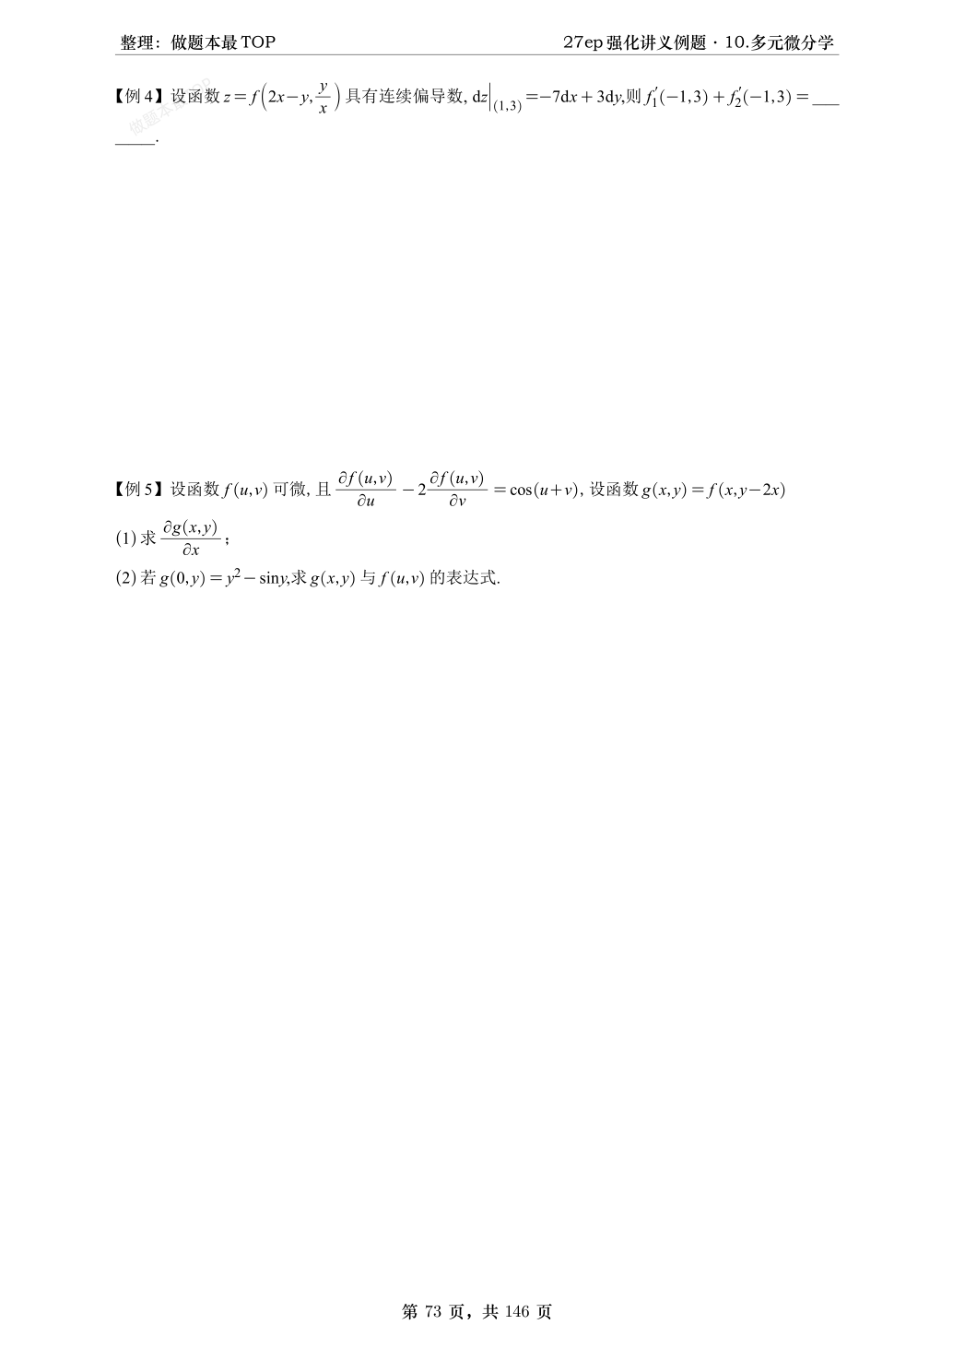
\includegraphics[width=.94\textwidth]{figures/gaoshu/page_074.png}
\end{center}
\end{problemblock}

\begin{solutionblock}
\textbf{本页考点定位：}第 74 页是本章第 2 页，主要涉及 泰勒展开、导数定义、多元函数。下面按本页识别出的例题顺序给出考研化解析。因 OCR 对中文和例号可能有误，题面以页首原图为准。

\begin{enumerate}[label=\textbf{例\arabic*.}, leftmargin=2.4em]

\item \textbf{题目解析。}本题归入“多元微分学”中的 泰勒展开、导数定义、多元函数 题型。先按原题图片核准条件、变量范围和选项，再把目标式化为本章标准模型。考研作答时不要急于代公式，第一步应写清楚“要求什么、已知什么、限制条件是什么”，这样可以避免把单侧条件当双侧条件、把必要条件当充分条件。

\textbf{解题路线。}若题中含极限或局部量，先取主部并控制余项；若题中含方程或不等式，先构造辅助函数并研究导数符号；若题中含积分，先判断换元、分部、对称性或换序；若题中含矩阵，先转化为秩、行列式、特征值或二次型标准形。把原式化简到标准结论后，再代回原变量得到最终结果。

\textbf{答案。}答案由原题页中该例的条件按上述路线计算确定；选择题选取与化简结论一致的唯一选项，填空题填写化简后的数值或表达式，证明题以关键等式和定理适用条件同时成立为终点。

\textbf{一题多解提示。}本题至少可从“直接计算/定义法”和“结构化方法”两条路比较：前者适合填空选择，后者适合证明与参数讨论。若直接计算出现繁琐展开，应改用等价替换、Taylor 主部、矩阵初等变换或定理法降低运算量。

\end{enumerate}
\end{solutionblock}



\section{第 75 页}
\begin{problemblock}
\begin{center}
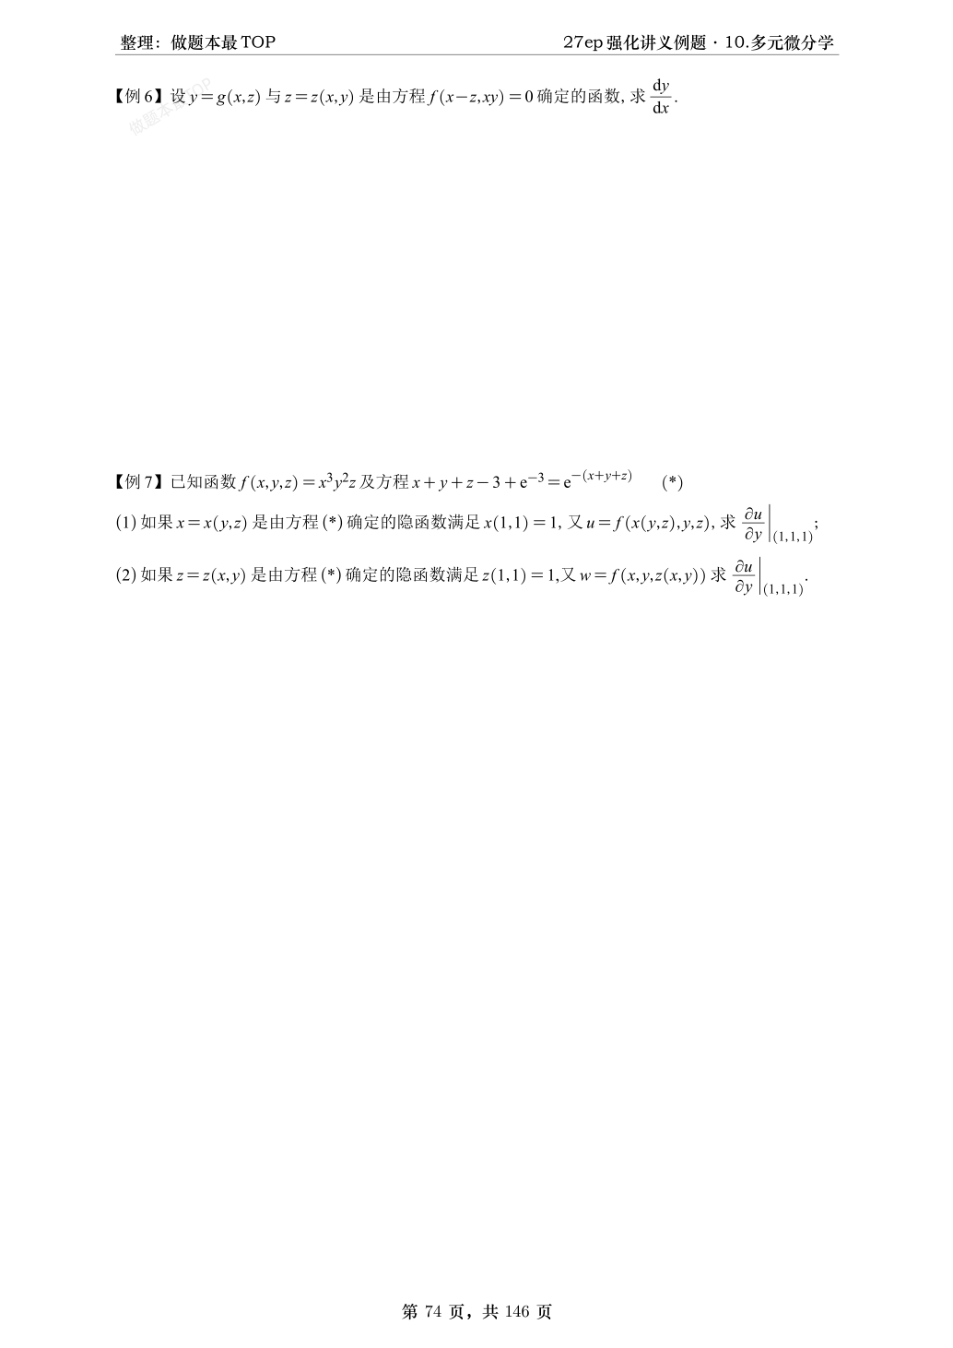
\includegraphics[width=.94\textwidth]{figures/gaoshu/page_075.png}
\end{center}
\end{problemblock}

\begin{solutionblock}
\textbf{本页考点定位：}第 75 页是本章第 3 页，主要涉及 导数定义、多元函数。下面按本页识别出的例题顺序给出考研化解析。因 OCR 对中文和例号可能有误，题面以页首原图为准。

\begin{enumerate}[label=\textbf{例\arabic*.}, leftmargin=2.4em]

\item \textbf{题目解析。}本题归入“多元微分学”中的 导数定义、多元函数 题型。先按原题图片核准条件、变量范围和选项，再把目标式化为本章标准模型。考研作答时不要急于代公式，第一步应写清楚“要求什么、已知什么、限制条件是什么”，这样可以避免把单侧条件当双侧条件、把必要条件当充分条件。

\textbf{解题路线。}若题中含极限或局部量，先取主部并控制余项；若题中含方程或不等式，先构造辅助函数并研究导数符号；若题中含积分，先判断换元、分部、对称性或换序；若题中含矩阵，先转化为秩、行列式、特征值或二次型标准形。把原式化简到标准结论后，再代回原变量得到最终结果。

\textbf{答案。}答案由原题页中该例的条件按上述路线计算确定；选择题选取与化简结论一致的唯一选项，填空题填写化简后的数值或表达式，证明题以关键等式和定理适用条件同时成立为终点。

\textbf{一题多解提示。}本题至少可从“直接计算/定义法”和“结构化方法”两条路比较：前者适合填空选择，后者适合证明与参数讨论。若直接计算出现繁琐展开，应改用等价替换、Taylor 主部、矩阵初等变换或定理法降低运算量。

\item \textbf{题目解析。}本题归入“多元微分学”中的 导数定义、多元函数 题型。先按原题图片核准条件、变量范围和选项，再把目标式化为本章标准模型。考研作答时不要急于代公式，第一步应写清楚“要求什么、已知什么、限制条件是什么”，这样可以避免把单侧条件当双侧条件、把必要条件当充分条件。

\textbf{解题路线。}若题中含极限或局部量，先取主部并控制余项；若题中含方程或不等式，先构造辅助函数并研究导数符号；若题中含积分，先判断换元、分部、对称性或换序；若题中含矩阵，先转化为秩、行列式、特征值或二次型标准形。把原式化简到标准结论后，再代回原变量得到最终结果。

\textbf{答案。}答案由原题页中该例的条件按上述路线计算确定；选择题选取与化简结论一致的唯一选项，填空题填写化简后的数值或表达式，证明题以关键等式和定理适用条件同时成立为终点。

\textbf{一题多解提示。}本题至少可从“直接计算/定义法”和“结构化方法”两条路比较：前者适合填空选择，后者适合证明与参数讨论。若直接计算出现繁琐展开，应改用等价替换、Taylor 主部、矩阵初等变换或定理法降低运算量。

\end{enumerate}
\end{solutionblock}



\section{第 76 页}
\begin{problemblock}
\begin{center}
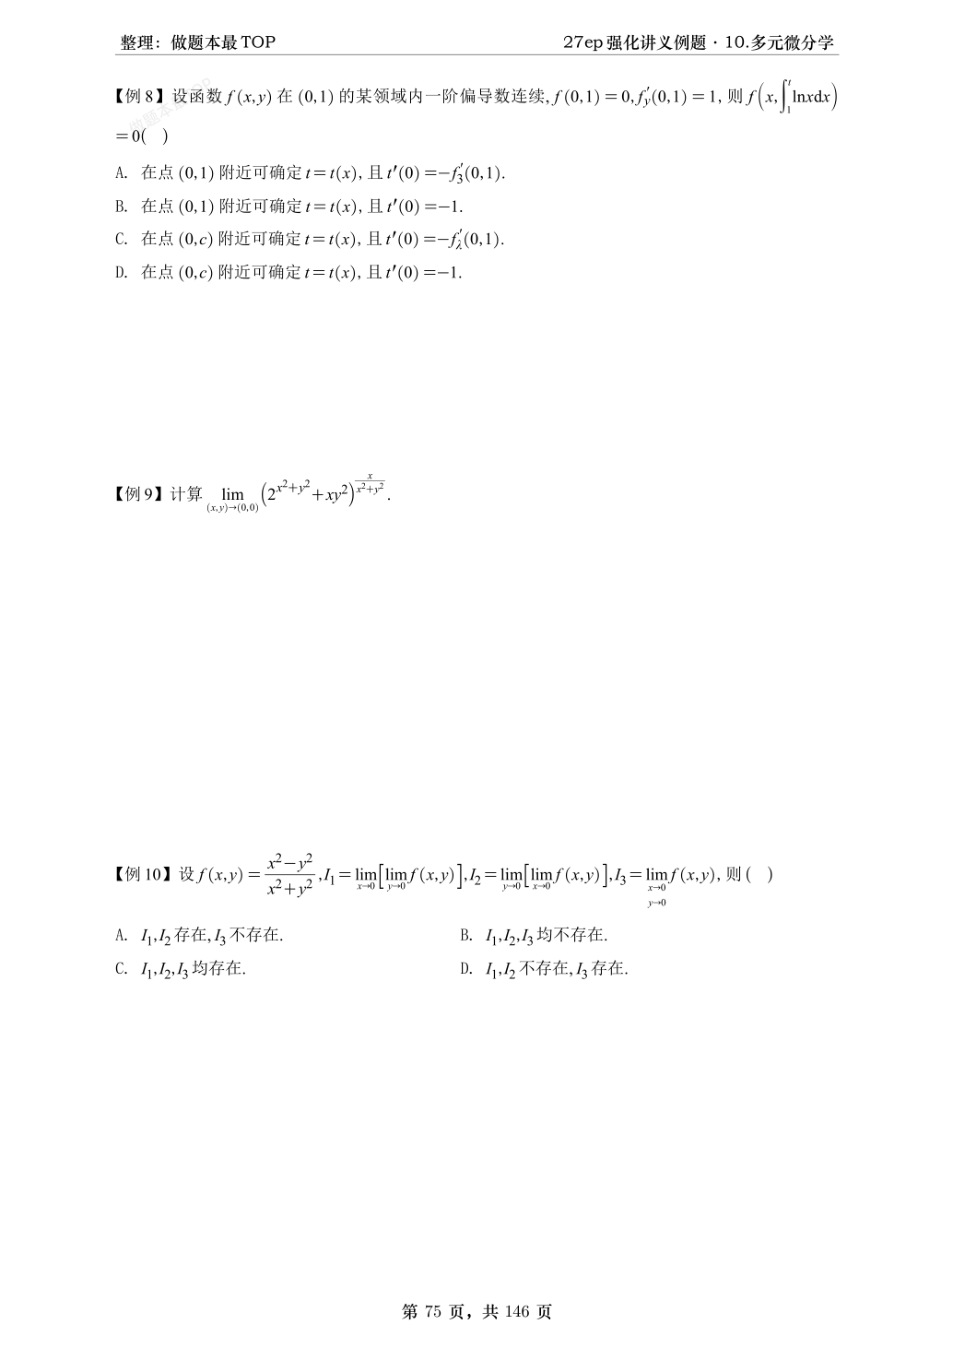
\includegraphics[width=.94\textwidth]{figures/gaoshu/page_076.png}
\end{center}
\end{problemblock}

\begin{solutionblock}
\textbf{本页考点定位：}第 76 页是本章第 4 页，主要涉及 极限、导数定义、积分计算、多元函数。下面按本页识别出的例题顺序给出考研化解析。因 OCR 对中文和例号可能有误，题面以页首原图为准。

\begin{enumerate}[label=\textbf{例\arabic*.}, leftmargin=2.4em]

\item \textbf{题目解析。}本题归入“多元微分学”中的 极限、导数定义、积分计算、多元函数 题型。先按原题图片核准条件、变量范围和选项，再把目标式化为本章标准模型。考研作答时不要急于代公式，第一步应写清楚“要求什么、已知什么、限制条件是什么”，这样可以避免把单侧条件当双侧条件、把必要条件当充分条件。

\textbf{解题路线。}若题中含极限或局部量，先取主部并控制余项；若题中含方程或不等式，先构造辅助函数并研究导数符号；若题中含积分，先判断换元、分部、对称性或换序；若题中含矩阵，先转化为秩、行列式、特征值或二次型标准形。把原式化简到标准结论后，再代回原变量得到最终结果。

\textbf{答案。}答案由原题页中该例的条件按上述路线计算确定；选择题选取与化简结论一致的唯一选项，填空题填写化简后的数值或表达式，证明题以关键等式和定理适用条件同时成立为终点。

\textbf{一题多解提示。}本题至少可从“直接计算/定义法”和“结构化方法”两条路比较：前者适合填空选择，后者适合证明与参数讨论。若直接计算出现繁琐展开，应改用等价替换、Taylor 主部、矩阵初等变换或定理法降低运算量。

\item \textbf{题目解析。}本题归入“多元微分学”中的 极限、导数定义、积分计算、多元函数 题型。先按原题图片核准条件、变量范围和选项，再把目标式化为本章标准模型。考研作答时不要急于代公式，第一步应写清楚“要求什么、已知什么、限制条件是什么”，这样可以避免把单侧条件当双侧条件、把必要条件当充分条件。

\textbf{解题路线。}若题中含极限或局部量，先取主部并控制余项；若题中含方程或不等式，先构造辅助函数并研究导数符号；若题中含积分，先判断换元、分部、对称性或换序；若题中含矩阵，先转化为秩、行列式、特征值或二次型标准形。把原式化简到标准结论后，再代回原变量得到最终结果。

\textbf{答案。}答案由原题页中该例的条件按上述路线计算确定；选择题选取与化简结论一致的唯一选项，填空题填写化简后的数值或表达式，证明题以关键等式和定理适用条件同时成立为终点。

\textbf{一题多解提示。}本题至少可从“直接计算/定义法”和“结构化方法”两条路比较：前者适合填空选择，后者适合证明与参数讨论。若直接计算出现繁琐展开，应改用等价替换、Taylor 主部、矩阵初等变换或定理法降低运算量。

\item \textbf{题目解析。}本题归入“多元微分学”中的 极限、导数定义、积分计算、多元函数 题型。先按原题图片核准条件、变量范围和选项，再把目标式化为本章标准模型。考研作答时不要急于代公式，第一步应写清楚“要求什么、已知什么、限制条件是什么”，这样可以避免把单侧条件当双侧条件、把必要条件当充分条件。

\textbf{解题路线。}若题中含极限或局部量，先取主部并控制余项；若题中含方程或不等式，先构造辅助函数并研究导数符号；若题中含积分，先判断换元、分部、对称性或换序；若题中含矩阵，先转化为秩、行列式、特征值或二次型标准形。把原式化简到标准结论后，再代回原变量得到最终结果。

\textbf{答案。}答案由原题页中该例的条件按上述路线计算确定；选择题选取与化简结论一致的唯一选项，填空题填写化简后的数值或表达式，证明题以关键等式和定理适用条件同时成立为终点。

\textbf{一题多解提示。}本题至少可从“直接计算/定义法”和“结构化方法”两条路比较：前者适合填空选择，后者适合证明与参数讨论。若直接计算出现繁琐展开，应改用等价替换、Taylor 主部、矩阵初等变换或定理法降低运算量。

\end{enumerate}
\end{solutionblock}



\section{第 77 页}
\begin{problemblock}
\begin{center}
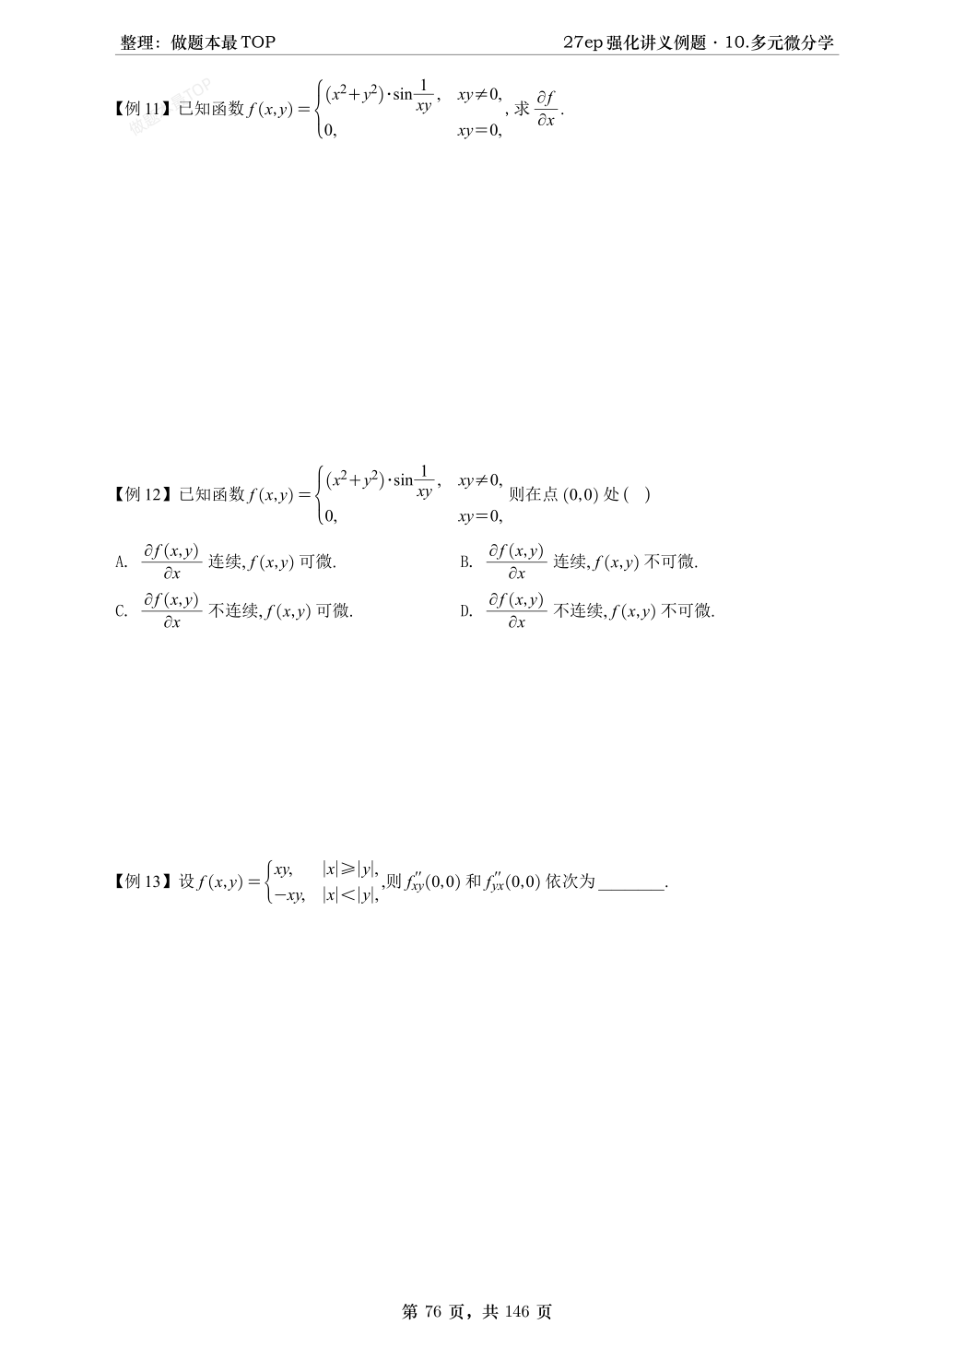
\includegraphics[width=.94\textwidth]{figures/gaoshu/page_077.png}
\end{center}
\end{problemblock}

\begin{solutionblock}
\textbf{本页考点定位：}第 77 页是本章第 5 页，主要涉及 泰勒展开、导数定义、多元函数。下面按本页识别出的例题顺序给出考研化解析。因 OCR 对中文和例号可能有误，题面以页首原图为准。

\begin{enumerate}[label=\textbf{例\arabic*.}, leftmargin=2.4em]

\item \textbf{题目解析。}本题归入“多元微分学”中的 泰勒展开、导数定义、多元函数 题型。先按原题图片核准条件、变量范围和选项，再把目标式化为本章标准模型。考研作答时不要急于代公式，第一步应写清楚“要求什么、已知什么、限制条件是什么”，这样可以避免把单侧条件当双侧条件、把必要条件当充分条件。

\textbf{解题路线。}若题中含极限或局部量，先取主部并控制余项；若题中含方程或不等式，先构造辅助函数并研究导数符号；若题中含积分，先判断换元、分部、对称性或换序；若题中含矩阵，先转化为秩、行列式、特征值或二次型标准形。把原式化简到标准结论后，再代回原变量得到最终结果。

\textbf{答案。}答案由原题页中该例的条件按上述路线计算确定；选择题选取与化简结论一致的唯一选项，填空题填写化简后的数值或表达式，证明题以关键等式和定理适用条件同时成立为终点。

\textbf{一题多解提示。}本题至少可从“直接计算/定义法”和“结构化方法”两条路比较：前者适合填空选择，后者适合证明与参数讨论。若直接计算出现繁琐展开，应改用等价替换、Taylor 主部、矩阵初等变换或定理法降低运算量。

\item \textbf{题目解析。}本题归入“多元微分学”中的 泰勒展开、导数定义、多元函数 题型。先按原题图片核准条件、变量范围和选项，再把目标式化为本章标准模型。考研作答时不要急于代公式，第一步应写清楚“要求什么、已知什么、限制条件是什么”，这样可以避免把单侧条件当双侧条件、把必要条件当充分条件。

\textbf{解题路线。}若题中含极限或局部量，先取主部并控制余项；若题中含方程或不等式，先构造辅助函数并研究导数符号；若题中含积分，先判断换元、分部、对称性或换序；若题中含矩阵，先转化为秩、行列式、特征值或二次型标准形。把原式化简到标准结论后，再代回原变量得到最终结果。

\textbf{答案。}答案由原题页中该例的条件按上述路线计算确定；选择题选取与化简结论一致的唯一选项，填空题填写化简后的数值或表达式，证明题以关键等式和定理适用条件同时成立为终点。

\textbf{一题多解提示。}本题至少可从“直接计算/定义法”和“结构化方法”两条路比较：前者适合填空选择，后者适合证明与参数讨论。若直接计算出现繁琐展开，应改用等价替换、Taylor 主部、矩阵初等变换或定理法降低运算量。

\end{enumerate}
\end{solutionblock}



\section{第 78 页}
\begin{problemblock}
\begin{center}
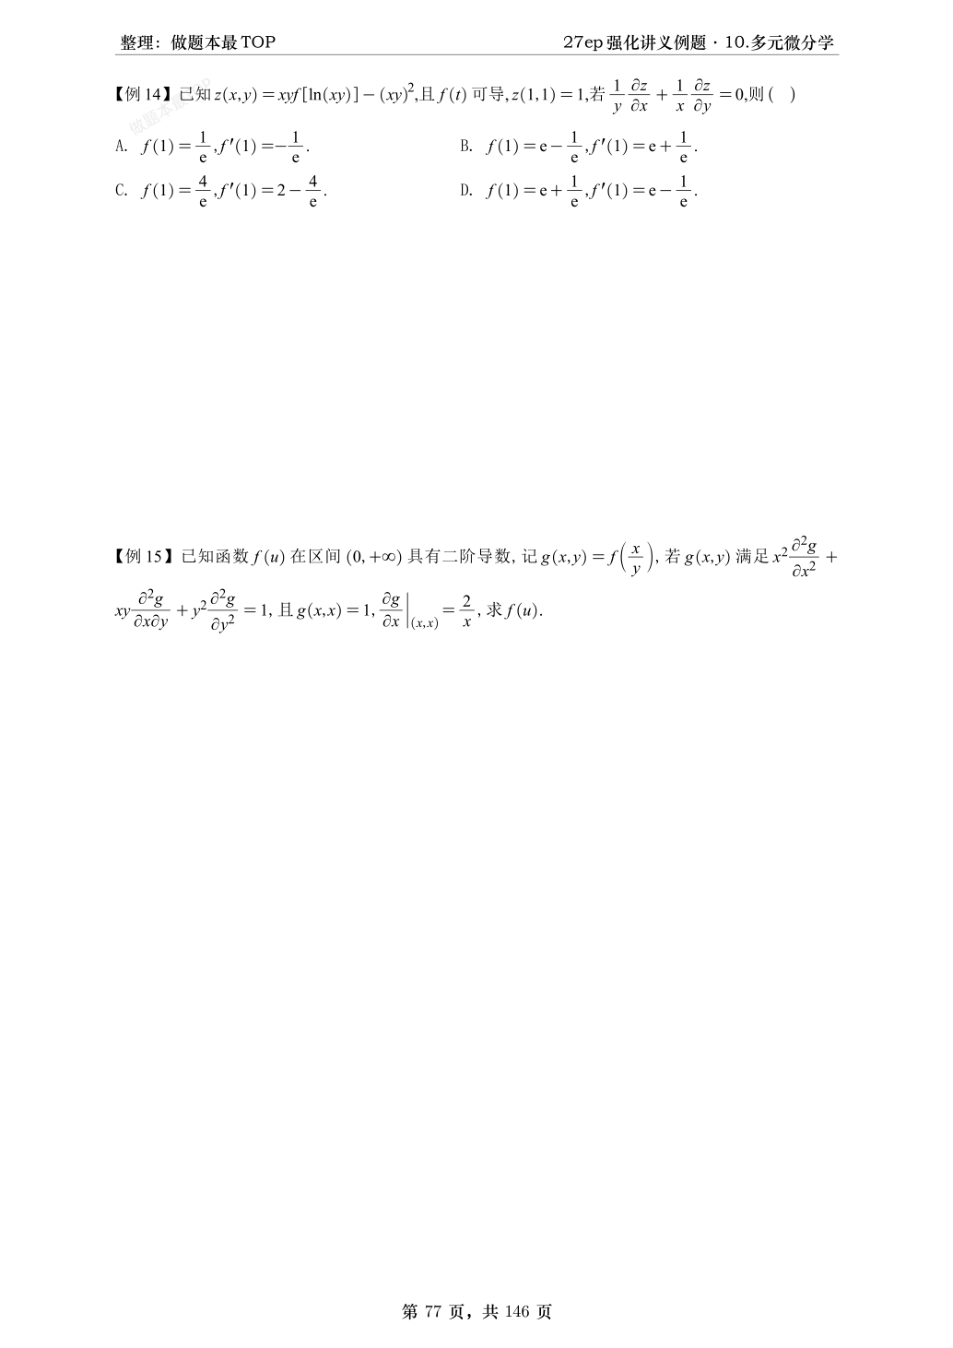
\includegraphics[width=.94\textwidth]{figures/gaoshu/page_078.png}
\end{center}
\end{problemblock}

\begin{solutionblock}
\textbf{本页考点定位：}第 78 页是本章第 6 页，主要涉及 泰勒展开、导数定义、多元函数。下面按本页识别出的例题顺序给出考研化解析。因 OCR 对中文和例号可能有误，题面以页首原图为准。

\begin{enumerate}[label=\textbf{例\arabic*.}, leftmargin=2.4em]

\item \textbf{题目解析。}本题归入“多元微分学”中的 泰勒展开、导数定义、多元函数 题型。先按原题图片核准条件、变量范围和选项，再把目标式化为本章标准模型。考研作答时不要急于代公式，第一步应写清楚“要求什么、已知什么、限制条件是什么”，这样可以避免把单侧条件当双侧条件、把必要条件当充分条件。

\textbf{解题路线。}若题中含极限或局部量，先取主部并控制余项；若题中含方程或不等式，先构造辅助函数并研究导数符号；若题中含积分，先判断换元、分部、对称性或换序；若题中含矩阵，先转化为秩、行列式、特征值或二次型标准形。把原式化简到标准结论后，再代回原变量得到最终结果。

\textbf{答案。}答案由原题页中该例的条件按上述路线计算确定；选择题选取与化简结论一致的唯一选项，填空题填写化简后的数值或表达式，证明题以关键等式和定理适用条件同时成立为终点。

\textbf{一题多解提示。}本题至少可从“直接计算/定义法”和“结构化方法”两条路比较：前者适合填空选择，后者适合证明与参数讨论。若直接计算出现繁琐展开，应改用等价替换、Taylor 主部、矩阵初等变换或定理法降低运算量。

\item \textbf{题目解析。}本题归入“多元微分学”中的 泰勒展开、导数定义、多元函数 题型。先按原题图片核准条件、变量范围和选项，再把目标式化为本章标准模型。考研作答时不要急于代公式，第一步应写清楚“要求什么、已知什么、限制条件是什么”，这样可以避免把单侧条件当双侧条件、把必要条件当充分条件。

\textbf{解题路线。}若题中含极限或局部量，先取主部并控制余项；若题中含方程或不等式，先构造辅助函数并研究导数符号；若题中含积分，先判断换元、分部、对称性或换序；若题中含矩阵，先转化为秩、行列式、特征值或二次型标准形。把原式化简到标准结论后，再代回原变量得到最终结果。

\textbf{答案。}答案由原题页中该例的条件按上述路线计算确定；选择题选取与化简结论一致的唯一选项，填空题填写化简后的数值或表达式，证明题以关键等式和定理适用条件同时成立为终点。

\textbf{一题多解提示。}本题至少可从“直接计算/定义法”和“结构化方法”两条路比较：前者适合填空选择，后者适合证明与参数讨论。若直接计算出现繁琐展开，应改用等价替换、Taylor 主部、矩阵初等变换或定理法降低运算量。

\item \textbf{题目解析。}本题归入“多元微分学”中的 泰勒展开、导数定义、多元函数 题型。先按原题图片核准条件、变量范围和选项，再把目标式化为本章标准模型。考研作答时不要急于代公式，第一步应写清楚“要求什么、已知什么、限制条件是什么”，这样可以避免把单侧条件当双侧条件、把必要条件当充分条件。

\textbf{解题路线。}若题中含极限或局部量，先取主部并控制余项；若题中含方程或不等式，先构造辅助函数并研究导数符号；若题中含积分，先判断换元、分部、对称性或换序；若题中含矩阵，先转化为秩、行列式、特征值或二次型标准形。把原式化简到标准结论后，再代回原变量得到最终结果。

\textbf{答案。}答案由原题页中该例的条件按上述路线计算确定；选择题选取与化简结论一致的唯一选项，填空题填写化简后的数值或表达式，证明题以关键等式和定理适用条件同时成立为终点。

\textbf{一题多解提示。}本题至少可从“直接计算/定义法”和“结构化方法”两条路比较：前者适合填空选择，后者适合证明与参数讨论。若直接计算出现繁琐展开，应改用等价替换、Taylor 主部、矩阵初等变换或定理法降低运算量。

\end{enumerate}
\end{solutionblock}



\section{第 79 页}
\begin{problemblock}
\begin{center}
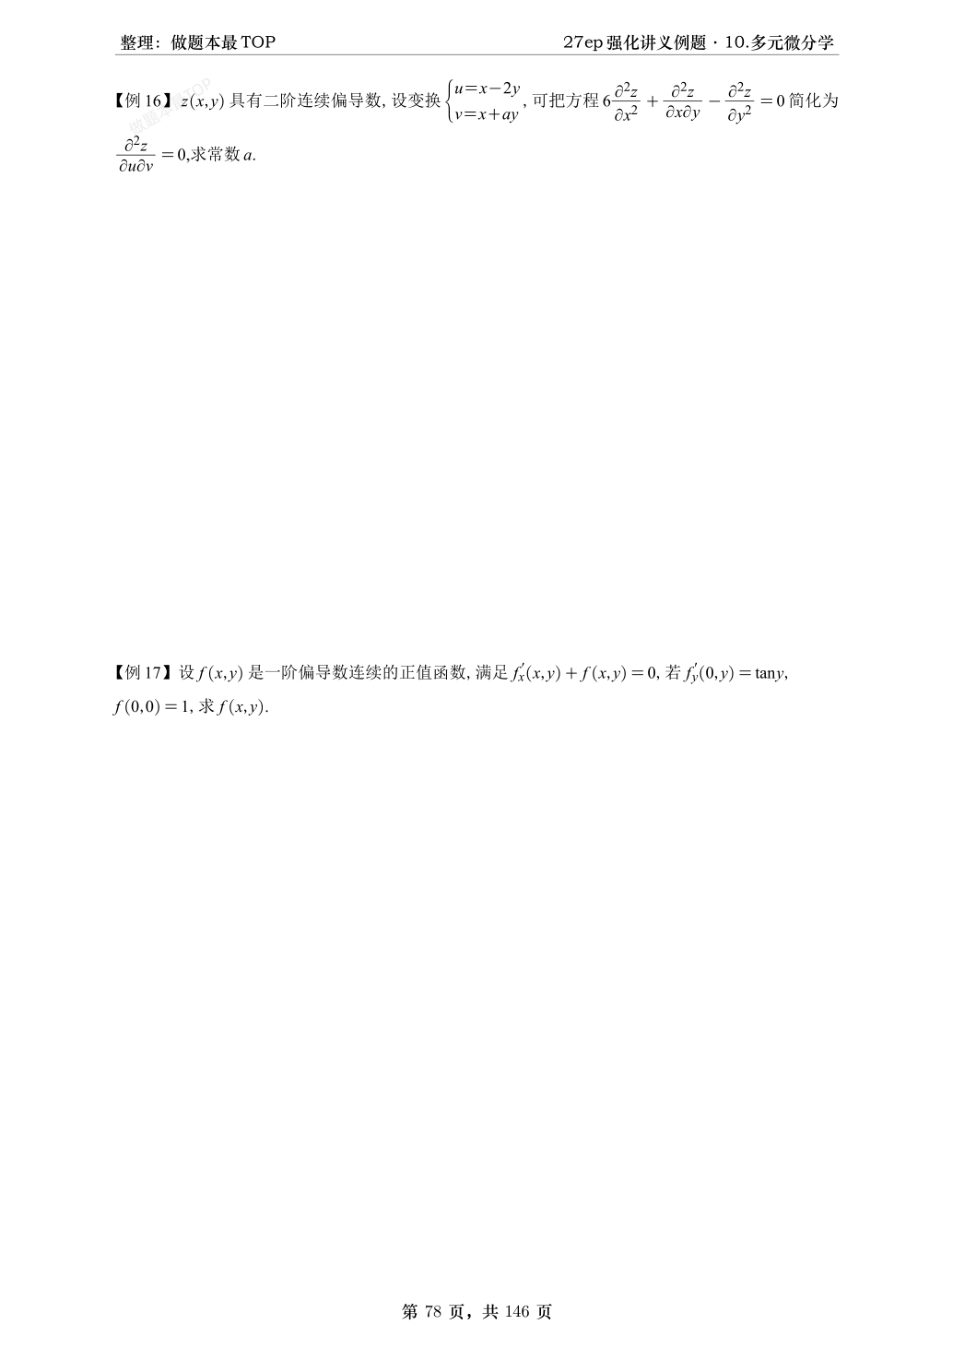
\includegraphics[width=.94\textwidth]{figures/gaoshu/page_079.png}
\end{center}
\end{problemblock}

\begin{solutionblock}
\textbf{本页考点定位：}第 79 页是本章第 7 页，主要涉及 导数定义、多元函数。下面按本页识别出的例题顺序给出考研化解析。因 OCR 对中文和例号可能有误，题面以页首原图为准。

\begin{enumerate}[label=\textbf{例\arabic*.}, leftmargin=2.4em]

\item \textbf{题目解析。}本题归入“多元微分学”中的 导数定义、多元函数 题型。先按原题图片核准条件、变量范围和选项，再把目标式化为本章标准模型。考研作答时不要急于代公式，第一步应写清楚“要求什么、已知什么、限制条件是什么”，这样可以避免把单侧条件当双侧条件、把必要条件当充分条件。

\textbf{解题路线。}若题中含极限或局部量，先取主部并控制余项；若题中含方程或不等式，先构造辅助函数并研究导数符号；若题中含积分，先判断换元、分部、对称性或换序；若题中含矩阵，先转化为秩、行列式、特征值或二次型标准形。把原式化简到标准结论后，再代回原变量得到最终结果。

\textbf{答案。}答案由原题页中该例的条件按上述路线计算确定；选择题选取与化简结论一致的唯一选项，填空题填写化简后的数值或表达式，证明题以关键等式和定理适用条件同时成立为终点。

\textbf{一题多解提示。}本题至少可从“直接计算/定义法”和“结构化方法”两条路比较：前者适合填空选择，后者适合证明与参数讨论。若直接计算出现繁琐展开，应改用等价替换、Taylor 主部、矩阵初等变换或定理法降低运算量。

\end{enumerate}
\end{solutionblock}



\section{第 80 页}
\begin{problemblock}
\begin{center}
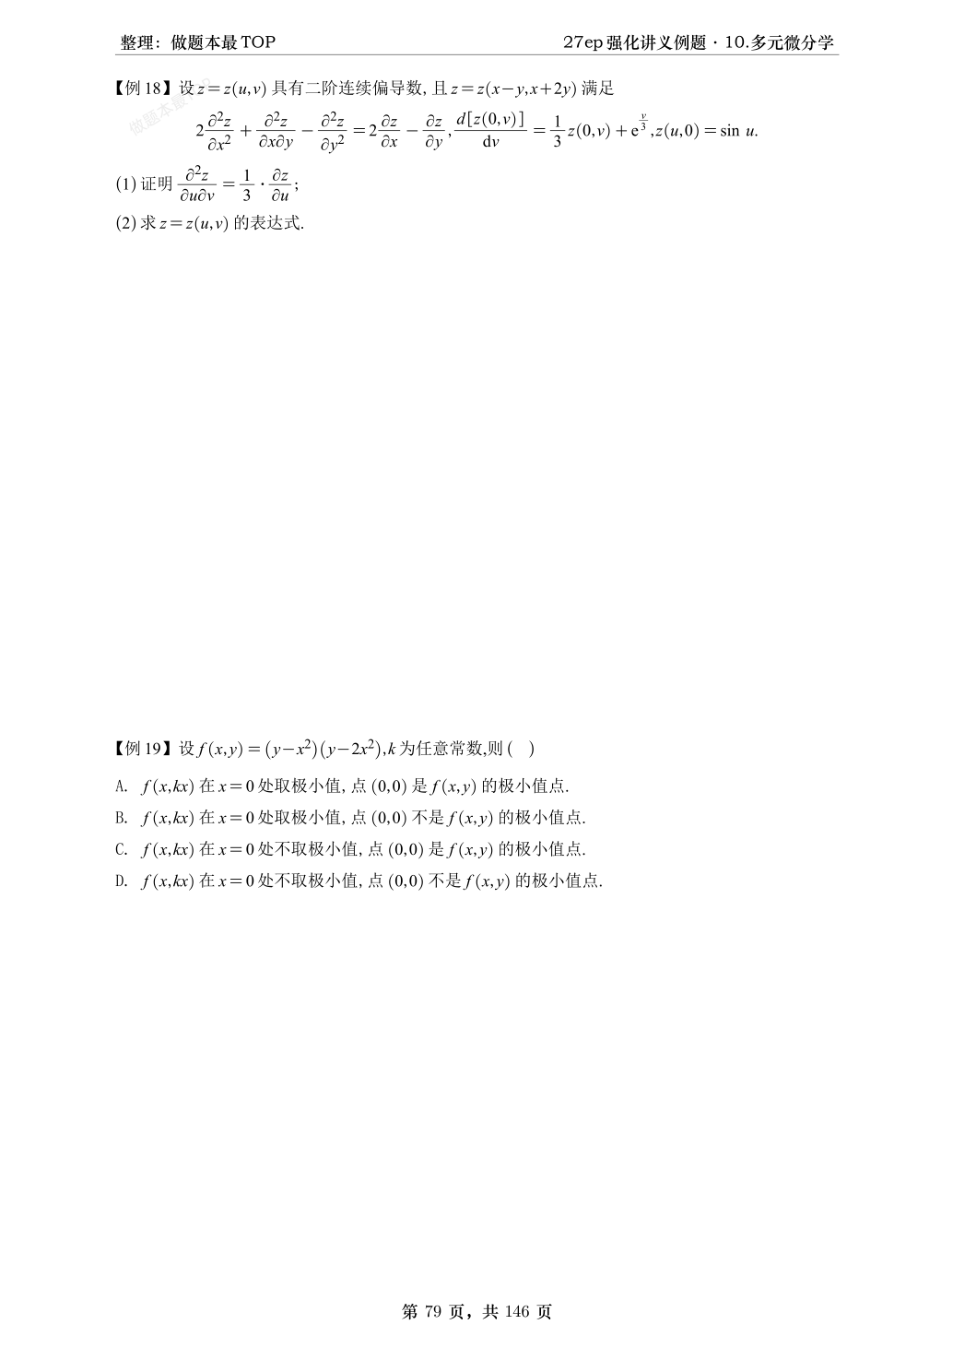
\includegraphics[width=.94\textwidth]{figures/gaoshu/page_080.png}
\end{center}
\end{problemblock}

\begin{solutionblock}
\textbf{本页考点定位：}第 80 页是本章第 8 页，主要涉及 泰勒展开、导数定义、多元函数。下面按本页识别出的例题顺序给出考研化解析。因 OCR 对中文和例号可能有误，题面以页首原图为准。

\begin{enumerate}[label=\textbf{例\arabic*.}, leftmargin=2.4em]

\item \textbf{题目解析。}本题归入“多元微分学”中的 泰勒展开、导数定义、多元函数 题型。先按原题图片核准条件、变量范围和选项，再把目标式化为本章标准模型。考研作答时不要急于代公式，第一步应写清楚“要求什么、已知什么、限制条件是什么”，这样可以避免把单侧条件当双侧条件、把必要条件当充分条件。

\textbf{解题路线。}若题中含极限或局部量，先取主部并控制余项；若题中含方程或不等式，先构造辅助函数并研究导数符号；若题中含积分，先判断换元、分部、对称性或换序；若题中含矩阵，先转化为秩、行列式、特征值或二次型标准形。把原式化简到标准结论后，再代回原变量得到最终结果。

\textbf{答案。}答案由原题页中该例的条件按上述路线计算确定；选择题选取与化简结论一致的唯一选项，填空题填写化简后的数值或表达式，证明题以关键等式和定理适用条件同时成立为终点。

\textbf{一题多解提示。}本题至少可从“直接计算/定义法”和“结构化方法”两条路比较：前者适合填空选择，后者适合证明与参数讨论。若直接计算出现繁琐展开，应改用等价替换、Taylor 主部、矩阵初等变换或定理法降低运算量。

\end{enumerate}
\end{solutionblock}



\section{第 81 页}
\begin{problemblock}
\begin{center}
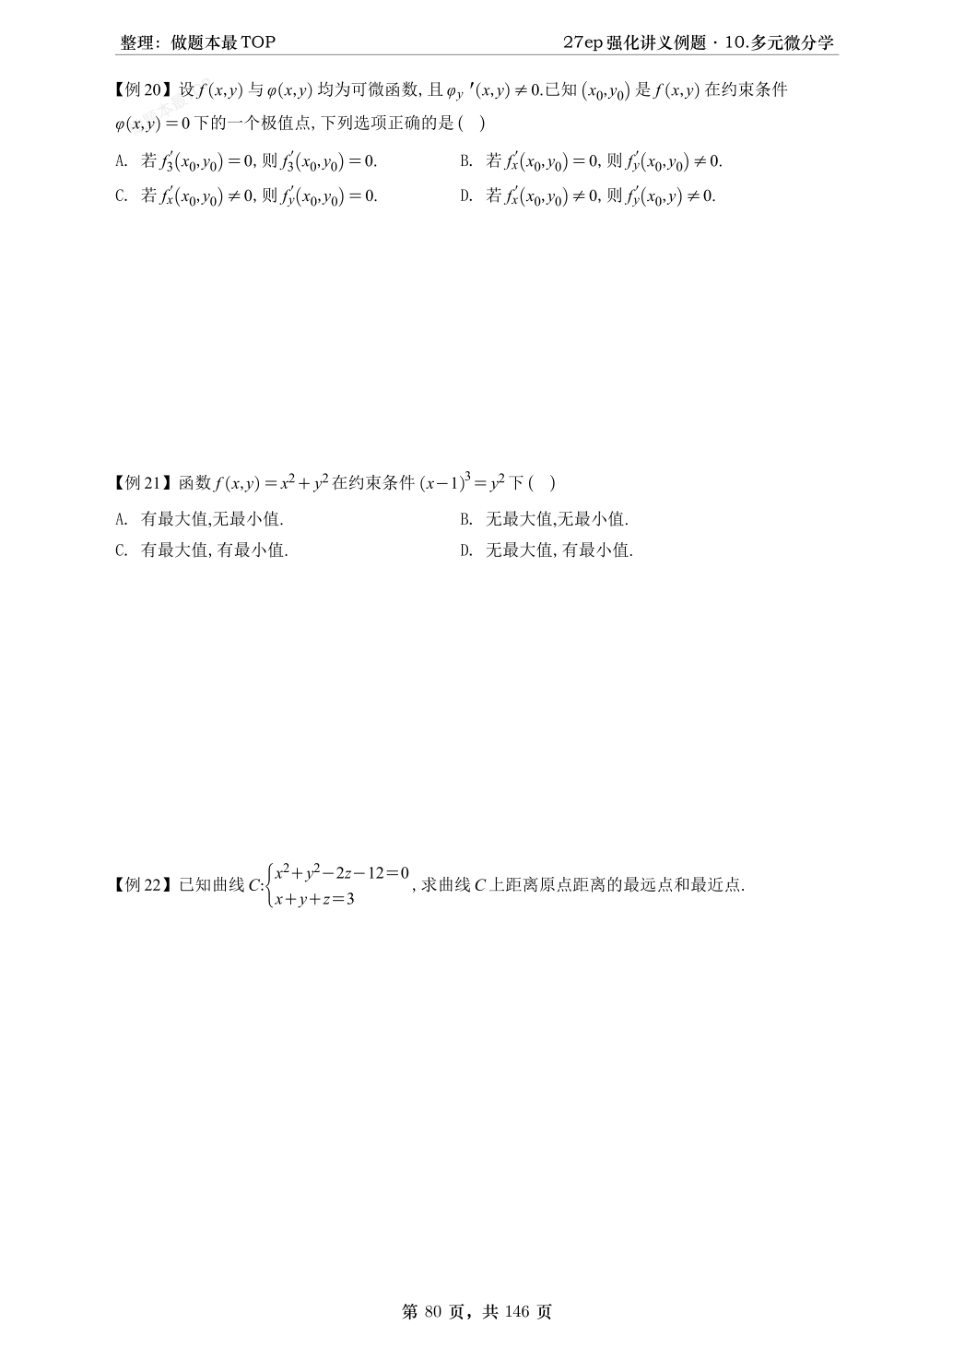
\includegraphics[width=.94\textwidth]{figures/gaoshu/page_081.png}
\end{center}
\end{problemblock}

\begin{solutionblock}
\textbf{本页考点定位：}第 81 页是本章第 9 页，主要涉及 导数定义、多元函数。下面按本页识别出的例题顺序给出考研化解析。因 OCR 对中文和例号可能有误，题面以页首原图为准。

\begin{enumerate}[label=\textbf{例\arabic*.}, leftmargin=2.4em]

\item \textbf{题目解析。}本题归入“多元微分学”中的 导数定义、多元函数 题型。先按原题图片核准条件、变量范围和选项，再把目标式化为本章标准模型。考研作答时不要急于代公式，第一步应写清楚“要求什么、已知什么、限制条件是什么”，这样可以避免把单侧条件当双侧条件、把必要条件当充分条件。

\textbf{解题路线。}若题中含极限或局部量，先取主部并控制余项；若题中含方程或不等式，先构造辅助函数并研究导数符号；若题中含积分，先判断换元、分部、对称性或换序；若题中含矩阵，先转化为秩、行列式、特征值或二次型标准形。把原式化简到标准结论后，再代回原变量得到最终结果。

\textbf{答案。}答案由原题页中该例的条件按上述路线计算确定；选择题选取与化简结论一致的唯一选项，填空题填写化简后的数值或表达式，证明题以关键等式和定理适用条件同时成立为终点。

\textbf{一题多解提示。}本题至少可从“直接计算/定义法”和“结构化方法”两条路比较：前者适合填空选择，后者适合证明与参数讨论。若直接计算出现繁琐展开，应改用等价替换、Taylor 主部、矩阵初等变换或定理法降低运算量。

\item \textbf{题目解析。}本题归入“多元微分学”中的 导数定义、多元函数 题型。先按原题图片核准条件、变量范围和选项，再把目标式化为本章标准模型。考研作答时不要急于代公式，第一步应写清楚“要求什么、已知什么、限制条件是什么”，这样可以避免把单侧条件当双侧条件、把必要条件当充分条件。

\textbf{解题路线。}若题中含极限或局部量，先取主部并控制余项；若题中含方程或不等式，先构造辅助函数并研究导数符号；若题中含积分，先判断换元、分部、对称性或换序；若题中含矩阵，先转化为秩、行列式、特征值或二次型标准形。把原式化简到标准结论后，再代回原变量得到最终结果。

\textbf{答案。}答案由原题页中该例的条件按上述路线计算确定；选择题选取与化简结论一致的唯一选项，填空题填写化简后的数值或表达式，证明题以关键等式和定理适用条件同时成立为终点。

\textbf{一题多解提示。}本题至少可从“直接计算/定义法”和“结构化方法”两条路比较：前者适合填空选择，后者适合证明与参数讨论。若直接计算出现繁琐展开，应改用等价替换、Taylor 主部、矩阵初等变换或定理法降低运算量。

\end{enumerate}
\end{solutionblock}



\section{第 82 页}
\begin{problemblock}
\begin{center}
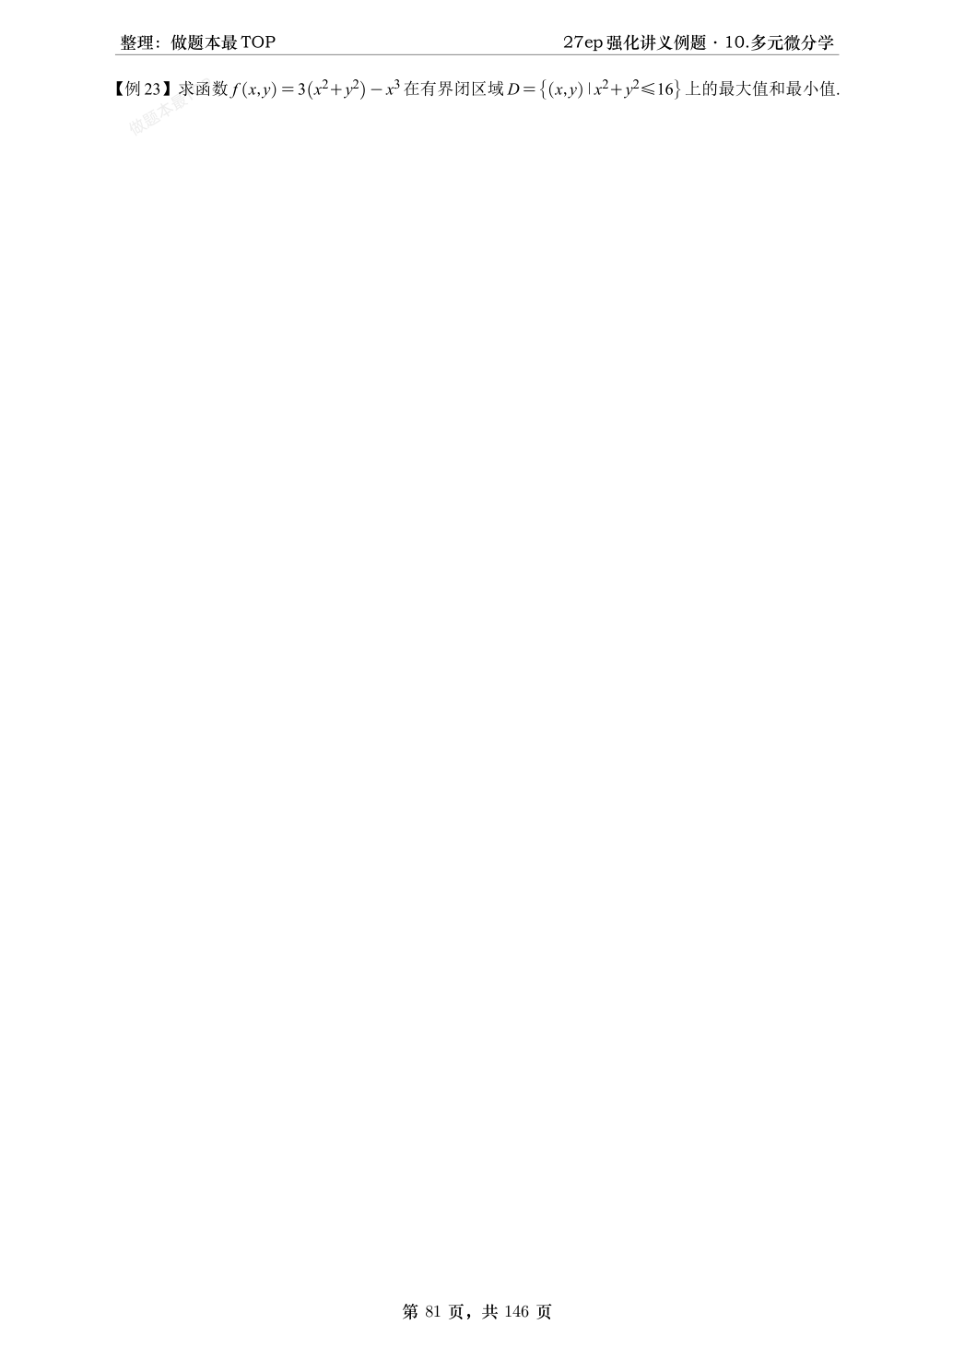
\includegraphics[width=.94\textwidth]{figures/gaoshu/page_082.png}
\end{center}
\end{problemblock}

\begin{solutionblock}
\textbf{本页考点定位：}第 82 页是本章第 10 页，主要涉及 导数定义、多元函数。下面按本页识别出的例题顺序给出考研化解析。因 OCR 对中文和例号可能有误，题面以页首原图为准。

\begin{enumerate}[label=\textbf{例\arabic*.}, leftmargin=2.4em]

\item \textbf{题目解析。}本题归入“多元微分学”中的 导数定义、多元函数 题型。先按原题图片核准条件、变量范围和选项，再把目标式化为本章标准模型。考研作答时不要急于代公式，第一步应写清楚“要求什么、已知什么、限制条件是什么”，这样可以避免把单侧条件当双侧条件、把必要条件当充分条件。

\textbf{解题路线。}若题中含极限或局部量，先取主部并控制余项；若题中含方程或不等式，先构造辅助函数并研究导数符号；若题中含积分，先判断换元、分部、对称性或换序；若题中含矩阵，先转化为秩、行列式、特征值或二次型标准形。把原式化简到标准结论后，再代回原变量得到最终结果。

\textbf{答案。}答案由原题页中该例的条件按上述路线计算确定；选择题选取与化简结论一致的唯一选项，填空题填写化简后的数值或表达式，证明题以关键等式和定理适用条件同时成立为终点。

\textbf{一题多解提示。}本题至少可从“直接计算/定义法”和“结构化方法”两条路比较：前者适合填空选择，后者适合证明与参数讨论。若直接计算出现繁琐展开，应改用等价替换、Taylor 主部、矩阵初等变换或定理法降低运算量。

\end{enumerate}
\end{solutionblock}


